%% =====================================================================
%%  2ª Avaliação — EECP0018 Processamento Digital de Sinais
%%  Formatação conforme ABNT (classe abntex2)
%% =====================================================================
\documentclass[
    12pt,
    openright,
    oneside,
    a4paper,
    chapter=TITLE,
    section=TITLE,
    brazil
]{abntex2}

\usepackage[T1]{fontenc}
\usepackage[utf8]{inputenc}
\usepackage{newtxtext,newtxmath}
\usepackage{amsmath, amssymb}
\usepackage{graphicx}
\usepackage{booktabs}
\usepackage{array}
\usepackage{microtype}
\usepackage{float}
\usepackage[alf]{abntex2cite}   % citações ABNT NBR 10520 (sistema autor-data)

% ---------------------------------------------------------------------
% Tamanho dos títulos: o padrão da classe (chapter=\Huge, section=\Large)
% foge do usual em trabalhos ABNT, em que a hierarquia é dada por
% numeração + negrito + caixa alta, não por fonte exagerada.
% ---------------------------------------------------------------------
\renewcommand{\ABNTEXchapterfontsize}{\large}
\renewcommand{\ABNTEXsectionfontsize}{\normalsize}
\renewcommand{\ABNTEXchapterfont}{\rmfamily}   % a classe usa \sffamily por padrão

\setlength{\afterchapskip}{1.0\baselineskip}

\hypersetup{hidelinks}

\def\clearforchapter{\relax}

\makeoddhead{abntheadings}{}{}{\ABNTEXfontereduzida\thepage}
\makeevenhead{abntheadings}{\ABNTEXfontereduzida\thepage}{}{}
\makeheadrule{abntheadings}{\textwidth}{0pt}

% ---------------------------------------------------------------------
% Dados do trabalho
% ---------------------------------------------------------------------
\titulo{Série de Fourier e Transformada de Fourier em Tempo Discreto:
        fundamentos, propriedades e aplicação computacional}
\autor{Ana Iara Loayza Costa\\José Victor Brito Costa\\Milena Freire Britto Neves}
\local{São Luís}
\data{2026}
\instituicao{Universidade Federal do Maranhão --- UFMA\\
             Centro de Ciências Exatas e Tecnologia\\
             Curso de Engenharia da Computação}
\tipotrabalho{Trabalho acadêmico}
\preambulo{Trabalho referente à 2ª Avaliação da disciplina EECP0018 --- Processamento
Digital de Sinais, do curso de Engenharia da Computação da Universidade Federal do
Maranhão, sob orientação do Prof. Dr. Pedro Baptista Fernandes.}

% ---------------------------------------------------------------------
% Capa personalizada com o brasão da UFMA
% ---------------------------------------------------------------------
\renewcommand{\imprimircapa}{%
  \begin{capa}
    \centering
    
\includegraphics[width=2.6cm]{images/ufma_logo.jpg}\par
    \vspace{0.6cm}
    {\ABNTEXchapterfont\large UNIVERSIDADE FEDERAL DO MARANHÃO\par}
    {\ABNTEXchapterfont CENTRO DE CIÊNCIAS EXATAS E TECNOLOGIA\par}
    {\ABNTEXchapterfont CURSO DE ENGENHARIA DA COMPUTAÇÃO\par}
    \vspace{2.5cm}
    {\ABNTEXchapterfont ANA IARA LOAYZA COSTA\par}
    {\ABNTEXchapterfont JOSÉ VICTOR BRITO COSTA\par}
    {\ABNTEXchapterfont MILENA FREIRE BRITTO NEVES\par}
    \vspace{3cm}
    {\ABNTEXchapterfont\bfseries\large SÉRIE DE FOURIER E TRANSFORMADA DE FOURIER
     EM TEMPO DISCRETO: FUNDAMENTOS, PROPRIEDADES E APLICAÇÃO COMPUTACIONAL\par}
    \vfill
    {\ABNTEXchapterfont São Luís\par}
    {\ABNTEXchapterfont 2026\par}
  \end{capa}
}

\begin{document}
\selectlanguage{brazil}
\frenchspacing

% =====================================================================
% ELEMENTOS PRÉ-TEXTUAIS
% =====================================================================
\pretextual
\imprimircapa
\imprimirfolhaderosto

\begin{resumo}
Este trabalho apresenta um estudo sobre a representação de sinais discretos no domínio
da frequência. São definidas a Série de Fourier em Tempo Discreto (SFTD), aplicável a
sinais periódicos, e a Transformada de Fourier em Tempo Discreto (TFTD), aplicável a
sinais aperiódicos, analisando-se comparativamente as características de seus espectros
quanto à natureza discreta ou contínua e à periodicidade. Em seguida, são sistematizadas
as principais propriedades da TFTD e estabelecida sua ligação com a transformada~$z$,
mostrando-se que a TFTD corresponde à avaliação da transformada~$z$ sobre a
circunferência unitária. Discute-se ainda a Transformada Rápida de Fourier (FFT) como
algoritmo eficiente para o cálculo da Transformada Discreta de Fourier (DFT), com
redução da complexidade de $O(N^2)$ para $O(N\log_2 N)$. Por fim, implementa-se em
Python o cálculo do espectro da TFTD de um pulso retangular de largura parametrizável,
obtendo-se o núcleo de Dirichlet e verificando-se numericamente a relação inversa entre
a duração do sinal no tempo e a largura do lóbulo principal em frequência. Os resultados
numéricos foram validados por três caminhos independentes de cálculo, com concordância
da ordem de $10^{-14}$.

\textbf{Palavras-chave}: processamento digital de sinais; transformada de Fourier;
tempo discreto; FFT; núcleo de Dirichlet.
\end{resumo}

\pdfbookmark[0]{\contentsname}{toc}
\tableofcontents*
\cleardoublepage

% =====================================================================
% ELEMENTOS TEXTUAIS
% =====================================================================
\textual

% ---------------------------------------------------------------------
\chapter{Introdução}

A análise de sinais no domínio da frequência é um dos pilares do processamento digital
de sinais. Enquanto a representação no tempo descreve quando os eventos ocorrem,
a representação em frequência revela de que componentes oscilatórias o sinal é
formado, informação essencial para projeto de filtros, compressão, modulação e
análise espectral \cite{oppenheim2013}.

Para sinais de tempo discreto, essa representação assume duas formas complementares,
conforme o sinal seja periódico ou aperiódico. Sinais periódicos são descritos pela
\textbf{Série de Fourier em Tempo Discreto} (SFTD), que os decompõe em um número
\emph{finito} de exponenciais complexas harmonicamente relacionadas. Sinais aperiódicos
de energia finita são descritos pela \textbf{Transformada de Fourier em Tempo Discreto}
(TFTD), que exige um \emph{contínuo} de frequências \cite{haykin1999}.

Este trabalho atende aos quatro tópicos solicitados no enunciado da avaliação. O
Capítulo~\ref{cap:sftd} define a SFTD e analisa seu espectro; o Capítulo~\ref{cap:tftd}
faz o mesmo para a TFTD e estabelece a comparação entre ambas; o
Capítulo~\ref{cap:propriedades} sistematiza as propriedades da TFTD; o
Capítulo~\ref{cap:z} demonstra sua ligação com a transformada~$z$; o
Capítulo~\ref{cap:fft} trata da Transformada Rápida de Fourier. Por fim, o
Capítulo~\ref{cap:aplicacao} apresenta a implementação computacional solicitada na
segunda questão, obtendo o espectro de um pulso retangular com largura parametrizável.

\newpage

% ---------------------------------------------------------------------
\chapter{Série de Fourier em Tempo Discreto}
\label{cap:sftd}

\section{Definição}

Seja $x[n]$ um sinal discreto \emph{periódico} de período fundamental $N$, isto é,
$x[n] = x[n+N]$ para todo $n$. Esse sinal pode ser representado como uma combinação
linear de exponenciais complexas harmonicamente relacionadas, cujas frequências são
múltiplas da frequência fundamental $\omega_0 = 2\pi/N$ \cite{haykin1999}.

A \textbf{equação de síntese} da SFTD é
\begin{equation}
    x[n] = \sum_{k=\langle N\rangle} a_k\, e^{\,jk\frac{2\pi}{N}n},
    \label{eq:sftd-sintese}
\end{equation}
e a \textbf{equação de análise}, que fornece os coeficientes espectrais, é
\begin{equation}
    a_k = \frac{1}{N}\sum_{n=\langle N\rangle} x[n]\, e^{-jk\frac{2\pi}{N}n},
    \label{eq:sftd-analise}
\end{equation}
onde a notação $\langle N\rangle$ indica que o somatório é feito sobre \emph{qualquer}
intervalo de $N$ amostras consecutivas.

\section{Características do espectro}

O espectro da SFTD, formado pelos coeficientes $a_k$, apresenta três características
determinantes:

\begin{alineas}
\item \textbf{É discreto.} O sinal é composto por um conjunto enumerável de raias
espectrais, localizadas nas frequências $\omega_k = k\,\frac{2\pi}{N}$. Não há
componentes em frequências intermediárias.

\item \textbf{É periódico em $k$, com período $N$.} Essa é uma diferença marcante em
relação ao caso contínuo. Como
\begin{equation}
    a_{k+N} = \frac{1}{N}\sum_{n=\langle N\rangle} x[n]\,e^{-j(k+N)\frac{2\pi}{N}n}
            = \frac{1}{N}\sum_{n=\langle N\rangle} x[n]\,e^{-jk\frac{2\pi}{N}n}
              \underbrace{e^{-j2\pi n}}_{=\,1} = a_k,
\end{equation}
os coeficientes se repetem. Consequentemente, existem apenas $N$ coeficientes
\emph{distintos}, e o somatório da Equação~\eqref{eq:sftd-sintese} é
\textbf{finito}, ao contrário da série de Fourier de tempo contínuo, que envolve
infinitos termos. Por isso a SFTD não apresenta problemas de convergência nem fenômeno
de Gibbs \cite{lathi2007}.

\item \textbf{Apresenta simetria hermitiana para sinais reais.} Se $x[n]$ é real, então
$a_{-k} = a_k^{*}$, de modo que a magnitude $|a_k|$ é uma função par e a fase
$\angle a_k$ é ímpar.
\end{alineas}

\vspace{1cm}

% ---------------------------------------------------------------------
\chapter{Transformada de Fourier em Tempo Discreto}
\label{cap:tftd}

\section{Definição e condições de existência}

Para sinais \emph{aperiódicos}, o espaçamento entre as raias espectrais
($2\pi/N$) tende a zero quando $N\to\infty$, e o espectro discreto transforma-se em uma
função contínua da frequência. Obtém-se assim o par de transformadas
\cite{oppenheim2013}:
\begin{equation}
    X(e^{j\omega}) = \sum_{n=-\infty}^{\infty} x[n]\,e^{-j\omega n}
    \qquad\text{(análise)},
    \label{eq:tftd-analise}
\end{equation}
\begin{equation}
    x[n] = \frac{1}{2\pi}\int_{2\pi} X(e^{j\omega})\,e^{j\omega n}\,d\omega
    \qquad\text{(síntese)}.
    \label{eq:tftd-sintese}
\end{equation}

A notação $X(e^{j\omega})$, em vez de $X(\omega)$, não é arbitrária: ela
antecipa a ligação com a transformada~$z$ discutida no Capítulo~\ref{cap:z}.

Quanto à existência, a série da Equação~\eqref{eq:tftd-analise} converge
\emph{uniformemente} se o sinal for absolutamente somável,
\begin{equation}
    \sum_{n=-\infty}^{\infty} |x[n]| < \infty,
\end{equation}
condição suficiente porém não necessária. Sinais de energia finita
($\sum |x[n]|^2 < \infty$) admitem TFTD no sentido da convergência em média
quadrática \cite{oppenheim1999}.

\section{Características do espectro}

\begin{alineas}
\item \textbf{É contínuo em $\omega$.} Diferentemente da SFTD, um sinal aperiódico
exige um contínuo de componentes de frequência para ser representado.

\item \textbf{É periódico com período $2\pi$.} Essa propriedade é intrínseca ao tempo
discreto. Como $n$ é inteiro,
\begin{equation}
    X\big(e^{j(\omega + 2\pi)}\big) = \sum_{n} x[n]\,e^{-j\omega n}
    \underbrace{e^{-j2\pi n}}_{=\,1} = X(e^{j\omega}).
\end{equation}
Toda a informação espectral está, portanto, contida em um intervalo de comprimento
$2\pi$, usualmente $-\pi < \omega \le \pi$. Nesse intervalo, $\omega = 0$ corresponde
às \emph{baixas} frequências e $\omega = \pm\pi$ às \emph{altas} frequências
\cite{oppenheim2013}.

\item \textbf{Apresenta simetria hermitiana para sinais reais.} Se $x[n]$ é real,
$X(e^{-j\omega}) = X^{*}(e^{j\omega})$; logo $|X(e^{j\omega})|$ é par e
$\angle X(e^{j\omega})$ é ímpar. Basta então representar $0 \le \omega \le \pi$.
\end{alineas}

\section{Comparação entre a SFTD e a TFTD}

O Quadro~\ref{quad:comparacao} sintetiza as diferenças. Observa-se a dualidade
característica da análise de Fourier: \emph{periodicidade em um domínio corresponde a
discretização no outro}.

\begin{table}[H]
\centering
\caption{Comparação entre a SFTD e a TFTD}
\label{quad:comparacao}
\begin{tabular}{@{}lll@{}}
\toprule
\textbf{Aspecto} & \textbf{SFTD} & \textbf{TFTD} \\
\midrule
Sinal no tempo        & periódico (período $N$)   & aperiódico \\
Natureza do espectro  & discreto (raias)          & contínuo em $\omega$ \\
Periodicidade         & periódico em $k$ ($N$)    & periódico em $\omega$ ($2\pi$) \\
Número de componentes & finito ($N$ distintos)    & infinito (não enumerável) \\
Operação de análise   & somatório finito          & somatório infinito \\
Operação de síntese   & somatório finito          & integral em $2\pi$ \\
Convergência          & sempre (soma finita)      & requer somabilidade \\
\bottomrule
\end{tabular}
\fonte{Elaborado pelos autores com base em \citeonline{oppenheim2013} e \citeonline{haykin1999}.}
\end{table}

% ---------------------------------------------------------------------
\chapter{Propriedades da TFTD}
\label{cap:propriedades}

As propriedades da TFTD são a base de quase toda manipulação prática de sinais: elas
permitem obter espectros de sinais compostos sem recorrer à definição. A
Tabela~\ref{tab:propriedades} reúne as principais, adotando-se a notação
$x[n] \longleftrightarrow X(e^{j\omega})$.

\begin{table}[H]
\centering
\caption{Principais propriedades da TFTD}
\label{tab:propriedades}
\small
\begin{tabular}{@{}p{4.6cm}p{3.5cm}p{5.9cm}@{}}
\toprule
\textbf{Propriedade} & \textbf{Sinal} & \textbf{Transformada} \\
\midrule
Linearidade &
$a\,x_1[n] + b\,x_2[n]$ &
$a\,X_1(e^{j\omega}) + b\,X_2(e^{j\omega})$ \\[2pt]

Deslocamento no tempo &
$x[n-n_d]$ &
$e^{-j\omega n_d}\,X(e^{j\omega})$ \\[2pt]

Deslocamento em frequência &
$e^{j\omega_0 n}\,x[n]$ &
$X\big(e^{j(\omega-\omega_0)}\big)$ \\[2pt]

Reversão no tempo &
$x[-n]$ &
$X(e^{-j\omega})$ \\[2pt]

Conjugação &
$x^{*}[n]$ &
$X^{*}(e^{-j\omega})$ \\[2pt]

Diferenciação em frequência &
$n\,x[n]$ &
$j\,\dfrac{dX(e^{j\omega})}{d\omega}$ \\[2pt]

Convolução &
$x[n] * h[n]$ &
$X(e^{j\omega})\,H(e^{j\omega})$ \\[2pt]

Multiplicação (janelamento) &
$x[n]\,w[n]$ &
$\dfrac{1}{2\pi}\displaystyle\int_{2\pi} X(e^{j\theta})\,W\big(e^{j(\omega-\theta)}\big)d\theta$ \\[2pt]

Teorema de Parseval &
\multicolumn{2}{l}{$\displaystyle\sum_{n=-\infty}^{\infty}|x[n]|^2
 = \frac{1}{2\pi}\int_{2\pi}\big|X(e^{j\omega})\big|^2 d\omega$} \\
\bottomrule
\end{tabular}
\fonte{Adaptado de \citeonline{oppenheim2013} e \citeonline{oppenheim1999}.}
\end{table}

Cada uma dessas propriedades é comentada a seguir, na ordem em que aparecem na
Tabela~\ref{tab:propriedades}.

\begin{alineas}
\item \textbf{Linearidade.} A TFTD é um operador linear: a transformada de uma
combinação linear de sinais é a mesma combinação linear das transformadas individuais.
É consequência direta da linearidade do somatório da Equação~\eqref{eq:tftd-analise} e
permite decompor um sinal complicado em parcelas mais simples, transformar cada uma
separadamente e somar os resultados \cite{oppenheim2013}.

\item \textbf{Deslocamento no tempo.} Um atraso $n_d$ não altera a magnitude do
espectro, apenas acrescenta uma fase linear $-\omega n_d$. Isso mostra que a informação
sobre a \emph{posição} do sinal no eixo do tempo está contida inteiramente na fase, e não
na magnitude, de $X(e^{j\omega})$.

\item \textbf{Deslocamento em frequência.} É a propriedade dual da anterior: multiplicar
o sinal por uma exponencial complexa $e^{j\omega_0 n}$ desloca todo o espectro de
$\omega_0$. É o princípio por trás da \emph{modulação}, usada para transportar um sinal
de banda base até uma faixa de frequências adequada à transmissão \cite{haykin1999}.

\item \textbf{Reversão no tempo.} Inverter a ordem das amostras no tempo reflete o
espectro em torno de $\omega = 0$. Para um sinal real, como já se tem
$X(e^{-j\omega}) = X^{*}(e^{j\omega})$ (simetria hermitiana), reverter o tempo produz o
mesmo efeito que conjugar o espectro.

\item \textbf{Conjugação.} Conjugar o sinal no tempo conjuga \emph{e} reflete o espectro
em frequência. Essa propriedade é a origem da simetria hermitiana discutida no
Capítulo~\ref{cap:tftd}: como um sinal real satisfaz $x^{*}[n] = x[n]$, aplicar a
propriedade a ambos os lados força $X^{*}(e^{-j\omega}) = X(e^{j\omega})$
\cite{oppenheim1999}.

\item \textbf{Diferenciação em frequência.} Ponderar o sinal por $n$ no tempo equivale a
derivar o espectro em relação a $\omega$. Essa propriedade é útil, por exemplo, para obter
o valor de $\sum n\,x[n]$ a partir da derivada de $X(e^{j\omega})$ em $\omega = 0$, sem
precisar recalcular o somatório.

\item \textbf{Convolução.} É a propriedade mais utilizada em processamento de sinais:
a convolução no tempo, operação custosa, corresponde a uma \emph{multiplicação} no
domínio da frequência. É o que fundamenta a filtragem digital, a saída de um sistema
LIT é obtida multiplicando-se o espectro da entrada pela resposta em frequência do
sistema \cite{lathi2007}.

\item \textbf{Multiplicação (janelamento).} É a propriedade dual da anterior:
multiplicar no tempo equivale a uma \emph{convolução periódica} em frequência. Ela
explica por que truncar um sinal (aplicar uma janela) provoca espalhamento espectral,
fenômeno observado diretamente nos lóbulos laterais do Capítulo~\ref{cap:aplicacao}.

\item \textbf{Teorema de Parseval.} Estabelece que a energia total do sinal, calculada
no tempo, é igual à energia calculada a partir do espectro, a menos do fator
$1/2\pi$, que vem da normalização da integral em um período de $2\pi$. É o que legitima
interpretar $|X(e^{j\omega})|^2$ como uma densidade de energia por unidade de frequência
\cite{oppenheim2013}.
\end{alineas}

\vspace{1cm}

% ---------------------------------------------------------------------
\chapter{Ligação entre a TFTD e a transformada \texorpdfstring{$z$}{z}}
\label{cap:z}

A transformada~$z$ bilateral de uma sequência $x[n]$ é definida por
\begin{equation}
    X(z) = \sum_{n=-\infty}^{\infty} x[n]\,z^{-n},
    \label{eq:z}
\end{equation}
sendo $z$ uma variável complexa. Escrevendo $z$ na forma polar, $z = r e^{j\omega}$,
e substituindo na Equação~\eqref{eq:z}:
\begin{equation}
    X(re^{j\omega}) = \sum_{n=-\infty}^{\infty}
        \big(x[n]\,r^{-n}\big)\,e^{-j\omega n}.
    \label{eq:z-polar}
\end{equation}

A Equação~\eqref{eq:z-polar} revela que a transformada~$z$ avaliada no raio $r$ é
exatamente a \textbf{TFTD da sequência ponderada} $x[n]\,r^{-n}$. O fator $r^{-n}$ atua
como uma exponencial de convergência: é ele que permite à transformada~$z$ existir para
sinais que não possuem TFTD, como o degrau unitário \cite{oppenheim1999}.

Fazendo $r = 1$, isto é, restringindo $z$ à \textbf{circunferência unitária}
$|z| = 1$, o fator de ponderação desaparece e obtém-se
\begin{equation}
    \boxed{\;X(e^{j\omega}) = X(z)\Big|_{z\,=\,e^{j\omega}}\;}
    \label{eq:ligacao}
\end{equation}

Ou seja: \textbf{a TFTD é a transformada~$z$ avaliada sobre a circunferência unitária}.
Desse resultado decorrem duas consequências importantes:

\begin{alineas}
\item \textbf{Condição de existência.} A TFTD de $x[n]$ existe se, e somente se, a
região de convergência (RDC) da transformada~$z$ \emph{contiver} a circunferência
unitária. Para um sistema causal com polos $p_i$, a RDC é $|z| > \max|p_i|$; logo, a
resposta em frequência existe se todos os polos estiverem no interior da circunferência
unitária, exatamente a condição de estabilidade BIBO \cite{oppenheim2013}.

\item \textbf{Interpretação geométrica.} Percorrer a circunferência unitária de
$\omega = -\pi$ a $\omega = \pi$ equivale a dar uma volta completa no plano~$z$. Isso
explica geometricamente a periodicidade de $2\pi$ da TFTD: após uma volta completa
retorna-se ao mesmo ponto. Além disso, a proximidade de um polo à circunferência produz
um pico na magnitude da resposta em frequência, enquanto a proximidade de um zero
produz uma depressão.
\end{alineas}

\vspace{1cm}

% ---------------------------------------------------------------------
\chapter{Transformada Rápida de Fourier}
\label{cap:fft}

\section{Da TFTD à DFT}

A TFTD, sendo função contínua de $\omega$, não pode ser calculada diretamente por um
computador: exigiria infinitos valores de frequência. A solução é \emph{amostrar} o
espectro em $N$ pontos igualmente espaçados, $\omega_k = 2\pi k/N$, o que define a
\textbf{Transformada Discreta de Fourier} (DFT) para uma sequência de comprimento
finito $N$ \cite{ingle2010}:
\begin{equation}
    X[k] = \sum_{n=0}^{N-1} x[n]\,e^{-j\frac{2\pi}{N}kn},
    \qquad k = 0,1,\dots,N-1.
    \label{eq:dft}
\end{equation}

Comparando as Equações~\eqref{eq:tftd-analise} e~\eqref{eq:dft}, verifica-se que
\begin{equation}
    X[k] = X(e^{j\omega})\Big|_{\omega\,=\,\frac{2\pi k}{N}},
\end{equation}
ou seja, \textbf{a DFT é uma versão amostrada da TFTD}. Essa relação é demonstrada
experimentalmente na Figura~\ref{fig:dftamostra}, no Capítulo~\ref{cap:aplicacao}.

\section{O algoritmo e o ganho computacional}

A \textbf{Transformada Rápida de Fourier} (FFT, de \emph{Fast Fourier Transform}) não é
uma transformada diferente: é um \emph{algoritmo eficiente} para calcular exatamente a
mesma DFT da Equação~\eqref{eq:dft}. O resultado é idêntico ao do cálculo direto, apenas se obtém muito mais rápido.

O cálculo direto da DFT exige, para cada um dos $N$ valores de $k$, um somatório de $N$
termos, resultando em $N^2$ multiplicações complexas: complexidade $O(N^2)$. O algoritmo
clássico, publicado por \citeonline{cooley1965}, explora a simetria e a periodicidade do
fator $W_N = e^{-j2\pi/N}$ por meio de uma estratégia de \emph{divisão e conquista}:
para $N$ potência de~2, a DFT de $N$ pontos é decomposta nas DFTs das amostras de
índice par e de índice ímpar, cada uma de $N/2$ pontos. Aplicando-se a decomposição
recursivamente, obtêm-se $\log_2 N$ estágios, cada um com $N/2$ operações elementares
(as chamadas \emph{borboletas}), o que leva à complexidade $O(N\log_2 N)$
\cite{oppenheim2013}.

A Tabela~\ref{tab:fft} quantifica a economia. Para $N = 4096$, a FFT é cerca de
683~vezes mais rápida, ganho que viabiliza aplicações em tempo real.

\begin{table}[H]
\centering
\caption{Multiplicações complexas: DFT direta \emph{versus} FFT (base 2)}
\label{tab:fft}
\begin{tabular}{@{}rrrr@{}}
\toprule
$N$ & DFT direta ($N^2$) & FFT ($\tfrac{N}{2}\log_2 N$) & Ganho \\
\midrule
    64 &        4.096 &    192 &  21,3$\times$ \\
   256 &       65.536 &  1.024 &  64,0$\times$ \\
 1.024 &    1.048.576 &  5.120 & 204,8$\times$ \\
 4.096 &   16.777.216 & 24.576 & 682,7$\times$ \\
\bottomrule
\end{tabular}
\fonte{Elaborado pelos autores.}
\end{table}

% ---------------------------------------------------------------------
\chapter{Aplicação: espectro da TFTD de um pulso retangular}
\label{cap:aplicacao}

\section{O sinal e o desenvolvimento analítico}

Conforme o enunciado, considera-se o pulso retangular de amplitude unitária
\begin{equation}
    x[n] = \begin{cases}
        1, & -4 \le n \le 4\\
        0, & \text{caso contrário,}
    \end{cases}
\end{equation}
que é o caso particular $M = 4$ da família generalizada
\begin{equation}
    x_M[n] = \begin{cases}
        1, & |n| \le M\\
        0, & \text{caso contrário,}
    \end{cases}
    \qquad L = 2M+1 \text{ amostras não nulas.}
\end{equation}

O sinal é mostrado na Figura~\ref{fig:sinal}.

\begin{figure}[H]
    \centering
    \caption{Pulso retangular $x[n]$ para $M = 4$}
    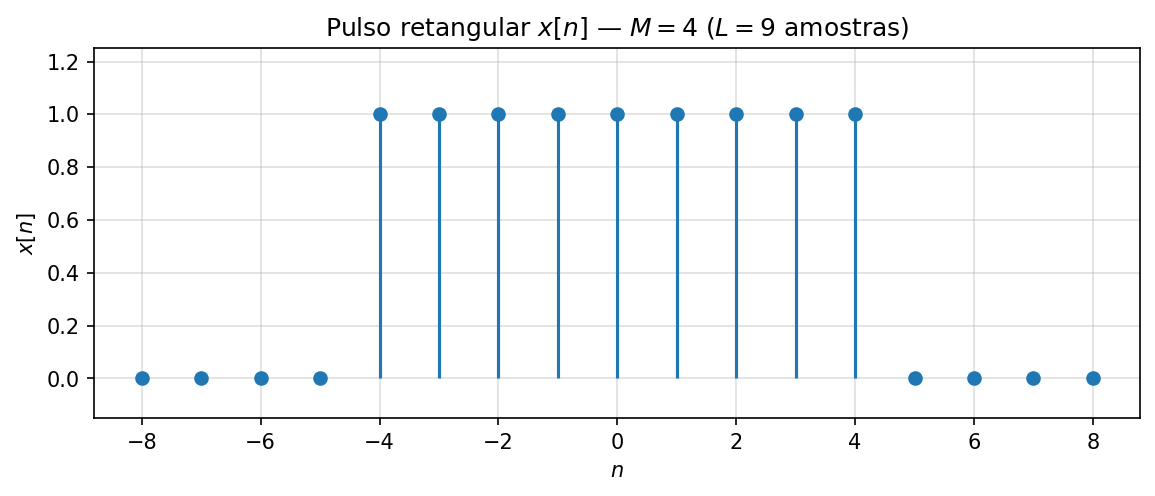
\includegraphics[width=0.78\textwidth]{images/sinal_tempo.png}
    \label{fig:sinal}
    \fonte{Elaborado pelos autores.}
\end{figure}

Aplicando a definição da Equação~\eqref{eq:tftd-analise}, o somatório se reduz ao
suporte finito do sinal:
\begin{equation}
    X_M(e^{j\omega}) = \sum_{n=-M}^{M} e^{-j\omega n}.
\end{equation}

Trata-se de uma progressão geométrica. Fazendo $r = e^{-j\omega}$ e multiplicando
numerador e denominador por $r^{-1/2}$ para simetrizar:
\begin{equation}
    \sum_{n=-M}^{M} r^{n}
    = \frac{r^{-M-\frac12} - r^{M+\frac12}}{r^{-\frac12} - r^{\frac12}}
    = \frac{e^{j\omega\left(M+\frac12\right)} - e^{-j\omega\left(M+\frac12\right)}}
           {e^{j\omega/2} - e^{-j\omega/2}}
    = \frac{2j\,\mathrm{sen}\!\left[\omega\!\left(M+\tfrac12\right)\right]}
           {2j\,\mathrm{sen}(\omega/2)}.
\end{equation}

Portanto,
\begin{equation}
    \boxed{\;X_M(e^{j\omega})
    = \frac{\mathrm{sen}\!\left(\dfrac{\omega L}{2}\right)}
           {\mathrm{sen}\!\left(\dfrac{\omega}{2}\right)},
    \qquad L = 2M+1\;}
    \label{eq:dirichlet}
\end{equation}
expressão conhecida como \textbf{núcleo de Dirichlet} ou \emph{sinc periódica}
\cite{oppenheim2013}. Dela decorrem as seguintes características:

\begin{alineas}
\item $X_M(e^{j\omega})$ é \textbf{puramente real}, consequência da simetria par do
sinal. A fase, portanto, só assume os valores $0$ (onde a função é positiva) e $\pi$
(onde é negativa);
\item em $\omega = 0$, o limite vale $X_M(e^{j0}) = L$, que é a soma de todas as
amostras;
\item os cruzamentos por zero ocorrem em $\omega = 2\pi k/L$, para $k$ inteiro não
múltiplo de $L$;
\item a \textbf{largura do lóbulo principal} é $4\pi/L$.
\end{alineas}

\section{Implementação}

O código foi desenvolvido em Python (bibliotecas \texttt{NumPy} e \texttt{Matplotlib}) e
encontra-se no arquivo \texttt{PDS\_ATV2.ipynb}. A largura é controlada pelo parâmetro
\texttt{M}, atendendo à exigência de generalização. O espectro é obtido por três
caminhos independentes, o que permite validação cruzada:

\begin{alineas}
\item \textbf{Pela definição}: avaliação direta do somatório
$\sum_n x[n]e^{-j\omega n}$, sem rotinas prontas;
\item \textbf{Pela forma fechada}: Equação~\eqref{eq:dirichlet};
\item \textbf{Pela FFT}: usando \texttt{numpy.fft.fft} com \emph{zero-padding},
conforme facultado pelo enunciado.
\end{alineas}

No cálculo via FFT, as amostras de índice negativo são posicionadas ao final do vetor,
respeitando a indexação circular assumida pela DFT. Esse cuidado preserva a fase e faz
com que o resultado saia real, como previsto pela teoria.

\section{Resultados}

A Figura~\ref{fig:espectro} apresenta o espectro obtido para $M = 4$. O painel superior
mostra $X(e^{j\omega})$ com sinal, sobreposto às amostras da FFT. O painel central mostra a magnitude, com o primeiro zero em
$\omega = \pm 2\pi/9 \approx \pm 0{,}698$~rad, e o inferior mostra a fase alternando
entre $0$ e $\pi$.

\begin{figure}[H]
    \centering
    \caption{Espectro da TFTD do pulso retangular ($M = 4$, $L = 9$)}
    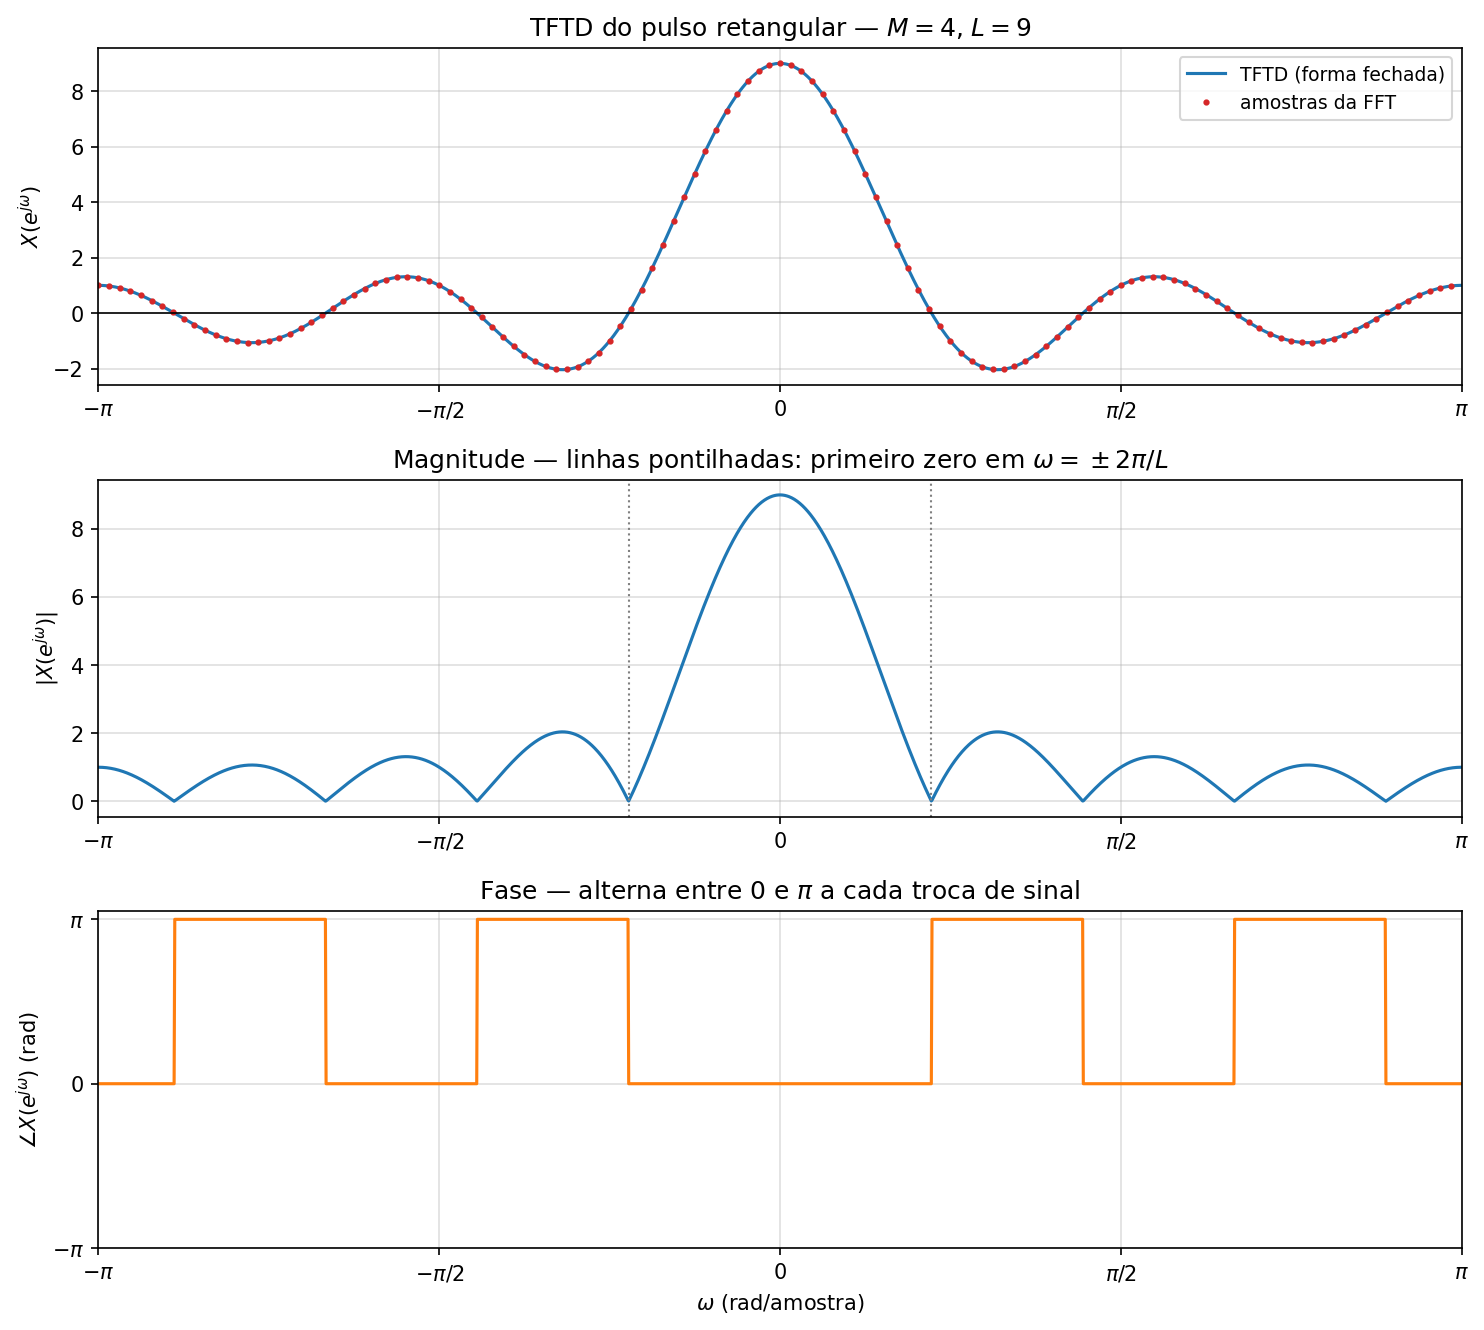
\includegraphics[width=0.86\textwidth]{images/espectro_M4.png}
    \label{fig:espectro}
    \fonte{Elaborado pelos autores.}
\end{figure}

A concordância numérica entre os três métodos é da ordem da precisão da máquina, e o
teorema de Parseval é verificado com erro de $1{,}78\times10^{-15}$, o que confirma a
correção da implementação.

\section{Generalização da largura}

A Figura~\ref{fig:largura} explora o efeito do parâmetro $M$. Observa-se a
\textbf{relação inversa} entre os domínios: quanto mais largo o pulso no tempo, mais
estreito o lóbulo principal em frequência. O pico central vale sempre $L = 2M+1$ e a
largura do lóbulo é $4\pi/L$, conforme a Tabela~\ref{tab:largura}.

\begin{figure}[H]
    \centering
    \caption{Efeito da largura do pulso sobre o espectro}
    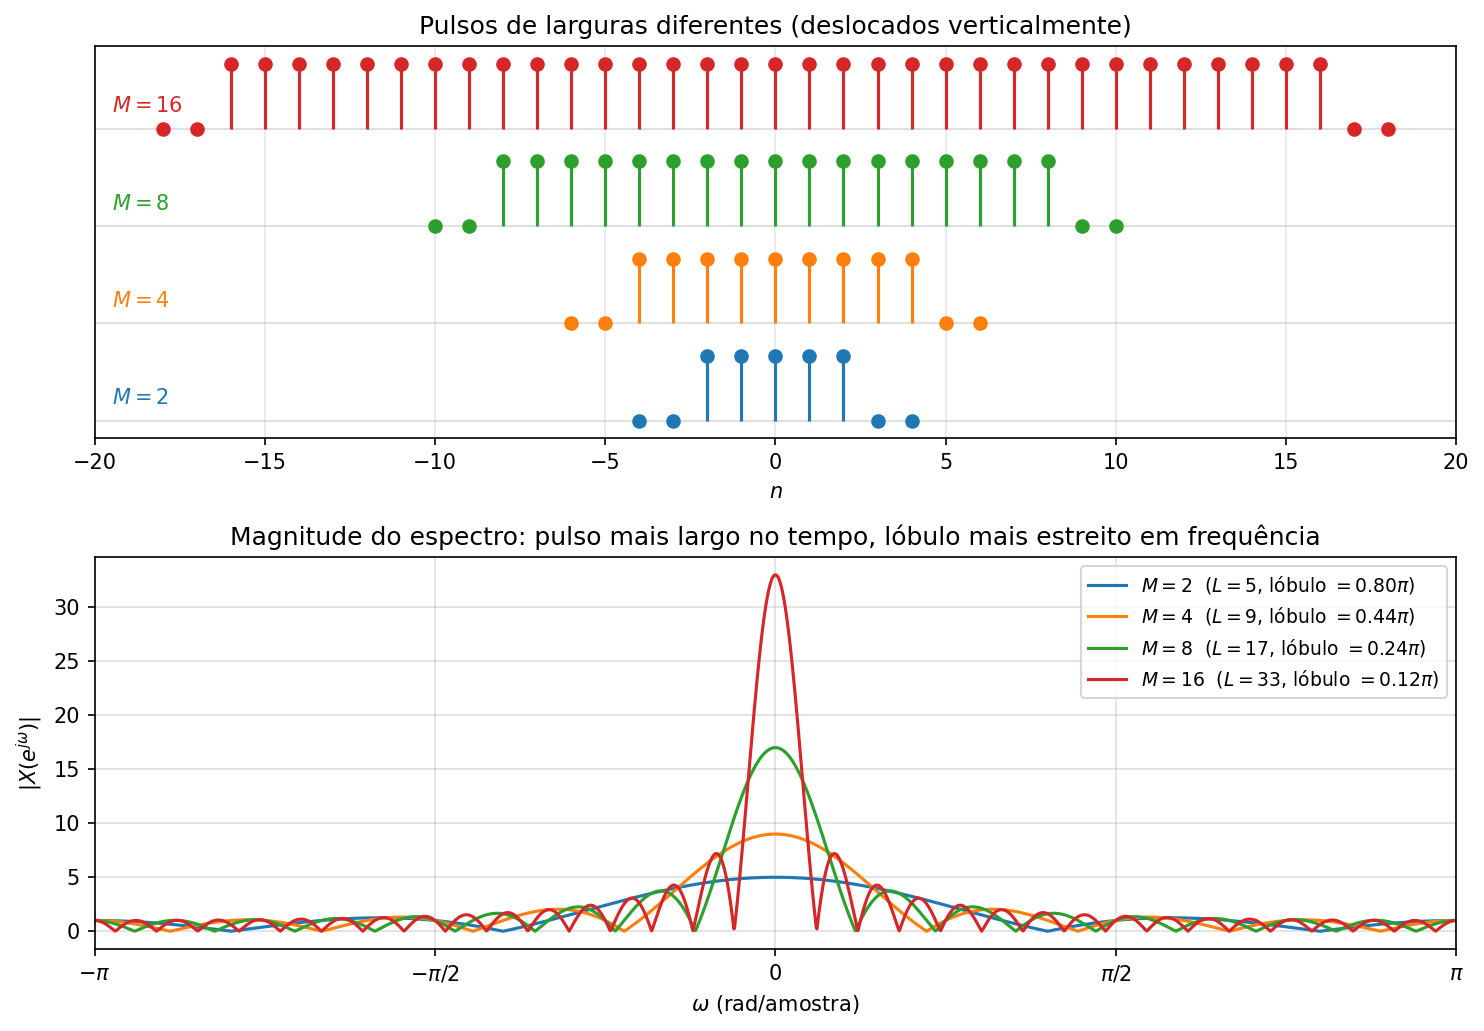
\includegraphics[width=0.86\textwidth]{images/efeito_largura.png}
    \label{fig:largura}
    \fonte{Elaborado pelos autores.}
\end{figure}

\begin{table}[H]
\centering
\caption{Relação entre a largura do pulso e o espectro}
\label{tab:largura}
\begin{tabular}{@{}rrrrr@{}}
\toprule
$M$ & $L = 2M+1$ & $X(e^{j0})$ & Primeiro zero & Lóbulo principal \\
\midrule
 2 &  5 &  5 & $0{,}400\pi$ & $0{,}800\pi$ \\
 4 &  9 &  9 & $0{,}222\pi$ & $0{,}444\pi$ \\
 8 & 17 & 17 & $0{,}118\pi$ & $0{,}235\pi$ \\
16 & 33 & 33 & $0{,}061\pi$ & $0{,}121\pi$ \\
\bottomrule
\end{tabular}
\fonte{Elaborado pelos autores.}
\end{table}

Essa é a manifestação discreta do princípio de que \emph{um sinal não pode ser
simultaneamente estreito no tempo e estreito em frequência}. No limite $M\to\infty$
(sinal constante), o espectro tenderia a um impulso em $\omega = 0$; no outro extremo,
$M = 0$ (impulso unitário), o espectro é constante e igual a~1, contendo todas as
frequências com o mesmo peso.

\section{A DFT como amostragem da TFTD}

Por fim, a Figura~\ref{fig:dftamostra} ilustra experimentalmente a relação discutida no
Capítulo~\ref{cap:fft}. Com $N$ pequeno, as amostras da DFT são esparsas; à medida que
$N$ cresce por \emph{zero-padding}, elas se adensam e reconstroem visualmente a curva
contínua da TFTD. É importante notar que o \emph{zero-padding} \textbf{não acrescenta
informação} ao sinal: apenas melhora a resolução gráfica do espectro.

\begin{figure}[H]
    \centering
    \caption{A DFT como amostragem da TFTD, para $N$ crescente}
    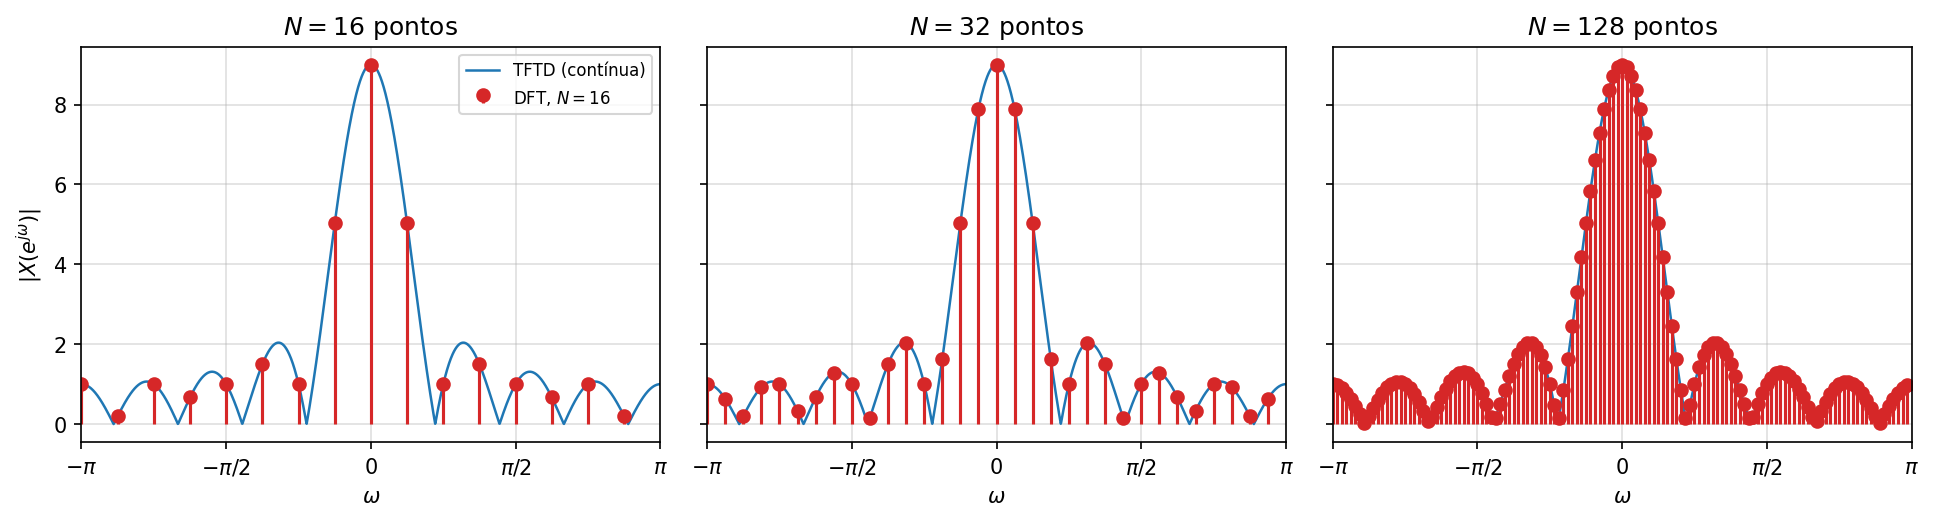
\includegraphics[width=\textwidth]{images/dft_amostra_tftd.png}
    \label{fig:dftamostra}
    \fonte{Elaborado pelos autores.}
\end{figure}

% ---------------------------------------------------------------------
\chapter{Conclusão}

Este trabalho percorreu as ferramentas de representação de sinais discretos no domínio
da frequência. Verificou-se que a SFTD e a TFTD são complementares: a primeira descreve
sinais periódicos por meio de um espectro \emph{discreto} e periódico em $k$, com apenas
$N$ componentes distintas; a segunda descreve sinais aperiódicos por meio de um espectro
\emph{contínuo} e periódico em $\omega$ com período $2\pi$. Em ambos os casos, a
periodicidade do espectro é uma marca do tempo discreto, sem contrapartida direta no
tempo contínuo.

As propriedades da TFTD, em especial a da convolução e sua dual, a da multiplicação, mostraram-se o elo entre a teoria e a prática da filtragem digital. A ligação com a
transformada~$z$ ficou estabelecida pela Equação~\eqref{eq:ligacao}: a TFTD é a
transformada~$z$ avaliada sobre a circunferência unitária, o que fornece, como
subproduto, o critério de existência da resposta em frequência e sua conexão direta com
a estabilidade do sistema.

Quanto à FFT, destacou-se que ela não é uma transformada distinta, mas um algoritmo que
calcula a DFT com complexidade $O(N\log_2 N)$ em vez de $O(N^2)$, ganho superior a
680 vezes já para $N = 4096$.

Na parte computacional, obteve-se o espectro do pulso retangular proposto, chegando-se
analiticamente ao núcleo de Dirichlet e confirmando-se o resultado por três caminhos
independentes, com erros da ordem de $10^{-14}$. A generalização da largura evidenciou a
relação inversa entre a duração no tempo e a ocupação em frequência, um dos princípios
mais fundamentais da análise de sinais.

\newpage

% =====================================================================
% ELEMENTOS PÓS-TEXTUAIS
% =====================================================================
\postextual
\bibliography{referencias}

\end{document}
